\documentclass[12pt,a4,english,finnish,pdflatex%,handout
]{beamer}
\definecolor{MyGreen}{RGB}{50, 120, 50}
\usecolortheme[named=MyGreen]{structure}

\usepackage{babel}
\usepackage[utf8]{inputenc}
\usepackage[T1]{fontenc}
\usepackage{amsmath,amssymb} 
\usepackage{animate}
\usepackage{multimedia}

\usepackage{natbib}
\bibpunct[: ]{(}{)}{,}{}{}{;}

\usepackage{tikz}

\usepackage{tipa}

\usepackage{hyperref}

\setbeamertemplate{navigation symbols}{}

\graphicspath{{figures/}}

\setlength{\leftmargini}{0pt}
\setlength{\leftmarginii}{1em}

%% Write out the names of graphics files being included 
\newwrite\graphics
\immediate\openout\graphics=\jobname.graphics%
\let\oincludegraphics\includegraphics% store original \includegraphics
\renewcommand{\includegraphics}[2][]{% prepend to it (could also use xpatch, etc.)
  \immediate\write\graphics{#2}
  \oincludegraphics[#1]{#2}}

\newcommand{\kommentti}[1]{
  {\bf[#1]}
}

\title{The process of initiating speech\\
and\\
The search for good analysis tools}
\author{Pertti Palo} 
\date{10 Mar 2025} 


\begin{document}

\frame{\titlepage
  \centering
} 

\frame{\frametitle{Land acknowledgement}
  I would like to respectfully acknowledge that we are located on Treaty 6
  territory, a traditional gathering place for diverse Indigenous peoples
  including the Cree, Blackfoot, Métis, Nakota Sioux, Iroquois, Dene, Ojibway/
  Saulteaux/Anishinaabe, Inuit, and many others. I am a very recent uninvited
  guest and I have only started learning about their histories, languages, and
  cultures and of their historical and continued contribution to our community.
  
  }

\frame{\frametitle{Outline}
  \begin{itemize}
    \item Introductions - Me and the topic
    \item Some naming experiments
    \item Some principles
    \item The tool: Pixel Difference (PD)
    \item Some quick results
    \item Conclusions
    % \item Second tool: Mean Squared Error (MSE)
  \end{itemize}
  \vfill
  {
  You can find these slides at: \url{https://github.com/giuthas-talks/McEwan2025/}
  }
}

\frame{\frametitle{Who's this Pertti Palo?}
  \begin{columns}
    \begin{column}{5cm}
      \includegraphics[width=\columnwidth]{uti_eva.png}
    \end{column}
    \begin{column}{5cm}
      \begin{itemize}
        \item I grew up in Finland, became me in Scotland and have since worked
        in Indiana and here in Edmonton.
        \item I have a couple of degrees in engineering and a PhD in Phonetics.
        \item I also have a life in folk music, folk dancing, oral
        storytelling, wandering (hiking and long distance skiing), role-playing
        games, crafts (knitting, terrain crafting, and other things).
      \end{itemize}
    \end{column}
  \end{columns}
} 

\frame{\frametitle{The topic}
  \begin{itemize}
  \item In my thesis I concentrated on timing of utterance onset in both
  acoustics and articulation \citep{Palo-MeasuringPrespeechArticulation-2019}.
  \item The data was high-speed tongue ultrasound from a delayed naming
  experiment -- specifically one using the Rastle instructions
  \citep{RastleEtAl-CharacterizingMotorExecution-2005}.
  \item For data analysis I need some new tools, but lets first talk about the
  data itself.
  \end{itemize} 

 	\centering
	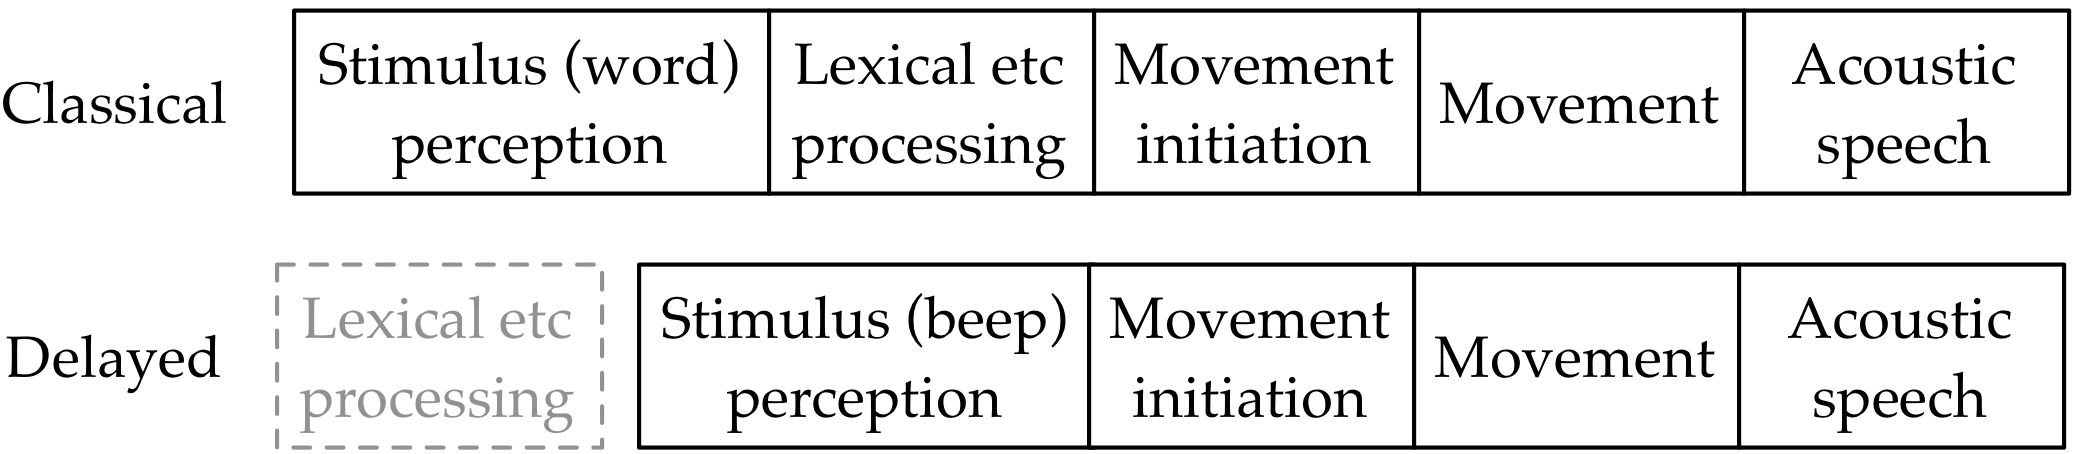
\includegraphics[width=\textwidth]{figures/stages_of_naming.jpg}
}


\frame{
  \centering
  {
    \bf \Large 
    \usebeamercolor[fg]{title}
    \vfill
    Some naming experiments
    
    \vfill
%    \includegraphics[height=1.5cm]{figures/aalto_logo} 
  }
}
\frame{\frametitle{Demo of classical naming}
  \begin{itemize}
    \item Let's try some versions of naming experiments.
  \item After the slide changes read out loud the word on the next slide as
  soon as you can.
  \end{itemize} 
}


\frame{
  \centering
  {
    \bf \Large 
    \usebeamercolor[fg]{title}
    \vfill
    red
    
    \vfill
%    \includegraphics[height=1.5cm]{figures/aalto_logo} 
  }
}

\frame{\frametitle{Demo of classical naming}
  \begin{itemize}
  \item Let's try that a second time.
  \end{itemize} 
}


\frame{
  \centering
  {
    \bf \Large 
    \usebeamercolor[fg]{title}
    \vfill
    green
    
    \vfill
%    \includegraphics[height=1.5cm]{figures/aalto_logo} 
  }
}

\frame{\frametitle{Demo of delayed naming}
  \begin{itemize}
  \item After the slide changes wait for me to snap my fingers.
  \item After you hear the finger snap, read the word out loud as soon as you
  can.
  \end{itemize} 
}


\frame{
  \centering
  {
    \bf \Large 
    \usebeamercolor[fg]{title}
    \vfill
    orange
    
    \vfill
%    \includegraphics[height=1.5cm]{figures/aalto_logo} 
  }
}

\frame{\frametitle{Demo of delayed naming}
  \begin{itemize}
  \item Rinse and repeat
  \end{itemize} 
}


\frame{
  \centering
  {
    \bf \Large 
    \usebeamercolor[fg]{title}
    \vfill
    purple
    
    \vfill
%    \includegraphics[height=1.5cm]{figures/aalto_logo} 
  }
}

\frame{\frametitle{Demo of delayed naming with Rastle instructions}
  \begin{itemize}
  \item After the slide changes wait \textbf{at rest} for me to snap my fingers.
  \item After you hear the finger snap, read the word out loud as soon as you
  can.
  \end{itemize} 
}


\frame{
  \centering
  {
    \bf \Large 
    \usebeamercolor[fg]{title}
    \vfill
    yellow
    
    \vfill
%    \includegraphics[height=1.5cm]{figures/aalto_logo} 
  }
}

\frame{\frametitle{Demo of delayed naming with Rastle instructions}
  \begin{itemize}
  \item Once more
  \end{itemize} 
}

\frame{
  \centering
  {
    \bf \Large 
    \usebeamercolor[fg]{title}
    \vfill
    blue
    
    \vfill
%    \includegraphics[height=1.5cm]{figures/aalto_logo} 
  }
}

\frame{\frametitle{What happened in the last one?}
  
  \begin{center}
    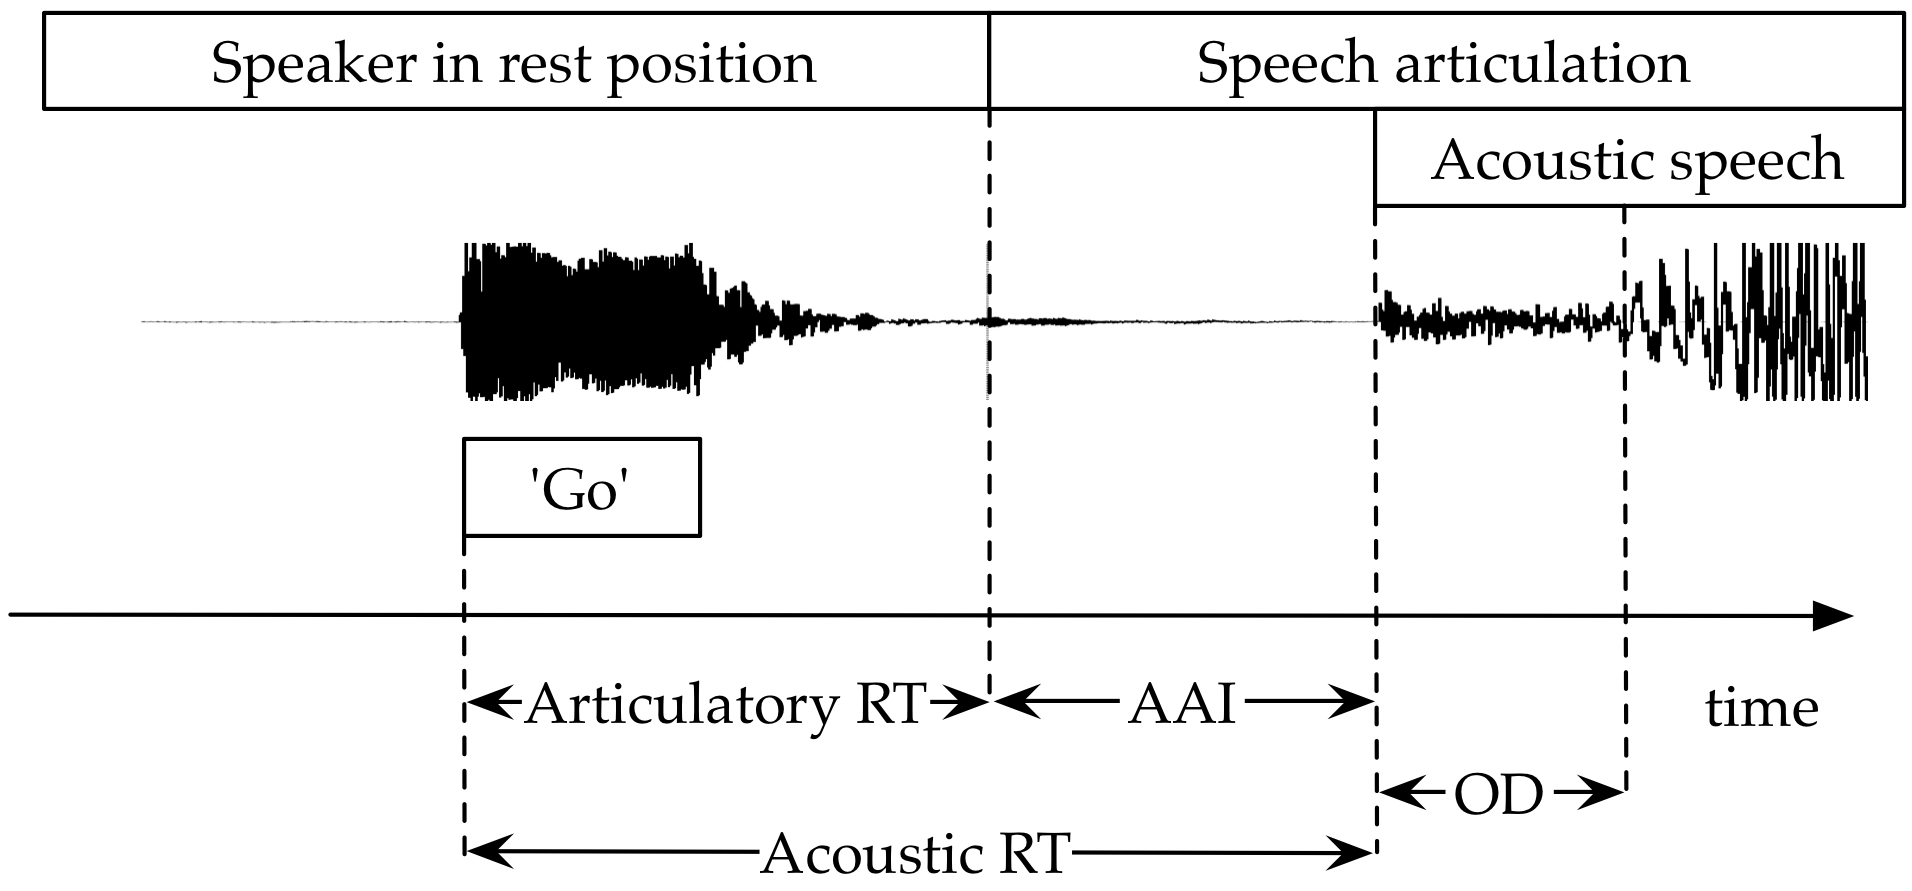
\includegraphics[width=\textwidth]{speech_prep_in_Rastle_task_annotated_long_names}
  \end{center}

  \begin{itemize}
  \item AAI = Articulatory onset to Acoustic onset Interval
  \item OD = Onset (or obstruent) Duration
  \end{itemize}
}

\frame{\frametitle{So what is the data actually like?}
  \begin{itemize}
    \item Now imagine that final experiment was recorded with tongue ultrasound
    imaging.
    \item And our job was to find the articulatory onset in the resulting
    greyscale videos.
    \item Here, let's try it. [external slide set coming up]
  \end{itemize} 
  }

\frame{\frametitle{And why new tools?}
  \begin{itemize}
    \item When trying to identify movement onset in greyscale videos with a lot
    of speckle 'noise', it doesn't take long to grow a desire for an easier way.
    \item The speckle 'noise' maybe caused by a number of factors including
    bubbles in the acoustic gel between the chin and the probe, noise sources in
    the equipment, and more interestingly changes in internal structures of
    tissues -- such as muscle fibres tensing and relaxing.
  \end{itemize}   
}

\frame{
  \centering
  {
    \vfill
    \bf \Large 
    \usebeamercolor[fg]{title}
    Some principles    
    \vfill
%    \includegraphics[height=1.5cm]{figures/aalto_logo} 
  }
}

\frame{\frametitle{Some principles I}
	\begin{itemize}
	\item When we are holding a hammer, everything looks like a nail.
	\item Every tool is a hammer\ldots
	\begin{itemize}
    \item \ldots at least until the first time we use it as a hammer\ldots
    \item \ldots which may lead to the item no longer being a tool at all.
	\end{itemize}
  \end{itemize}
}

\frame{\frametitle{Some principles II}
\begin{itemize}
  \item The first thing to do is to figure out if the tools we have match the
  question and data we have.
  \item And then get the right tool for the job, if we aren't lucky to begin
  with.
  \item Keeping in mind that 'good' is usually better than 'best'.
\end{itemize}
}

\frame{
  \centering
  {
    \vfill
    \bf \Large 
    \usebeamercolor[fg]{title}
    The tool: Pixel Difference (PD)    
    \vfill
%    \includegraphics[height=1.5cm]{figures/aalto_logo} 
  }
}

\frame{\frametitle{Pixel Difference (PD)}
	\begin{itemize}
    \item The first tool out of the box was manual video segmentation.
    \item The second tool out of the box happened to work much better.
	\end{itemize}


	\centering
	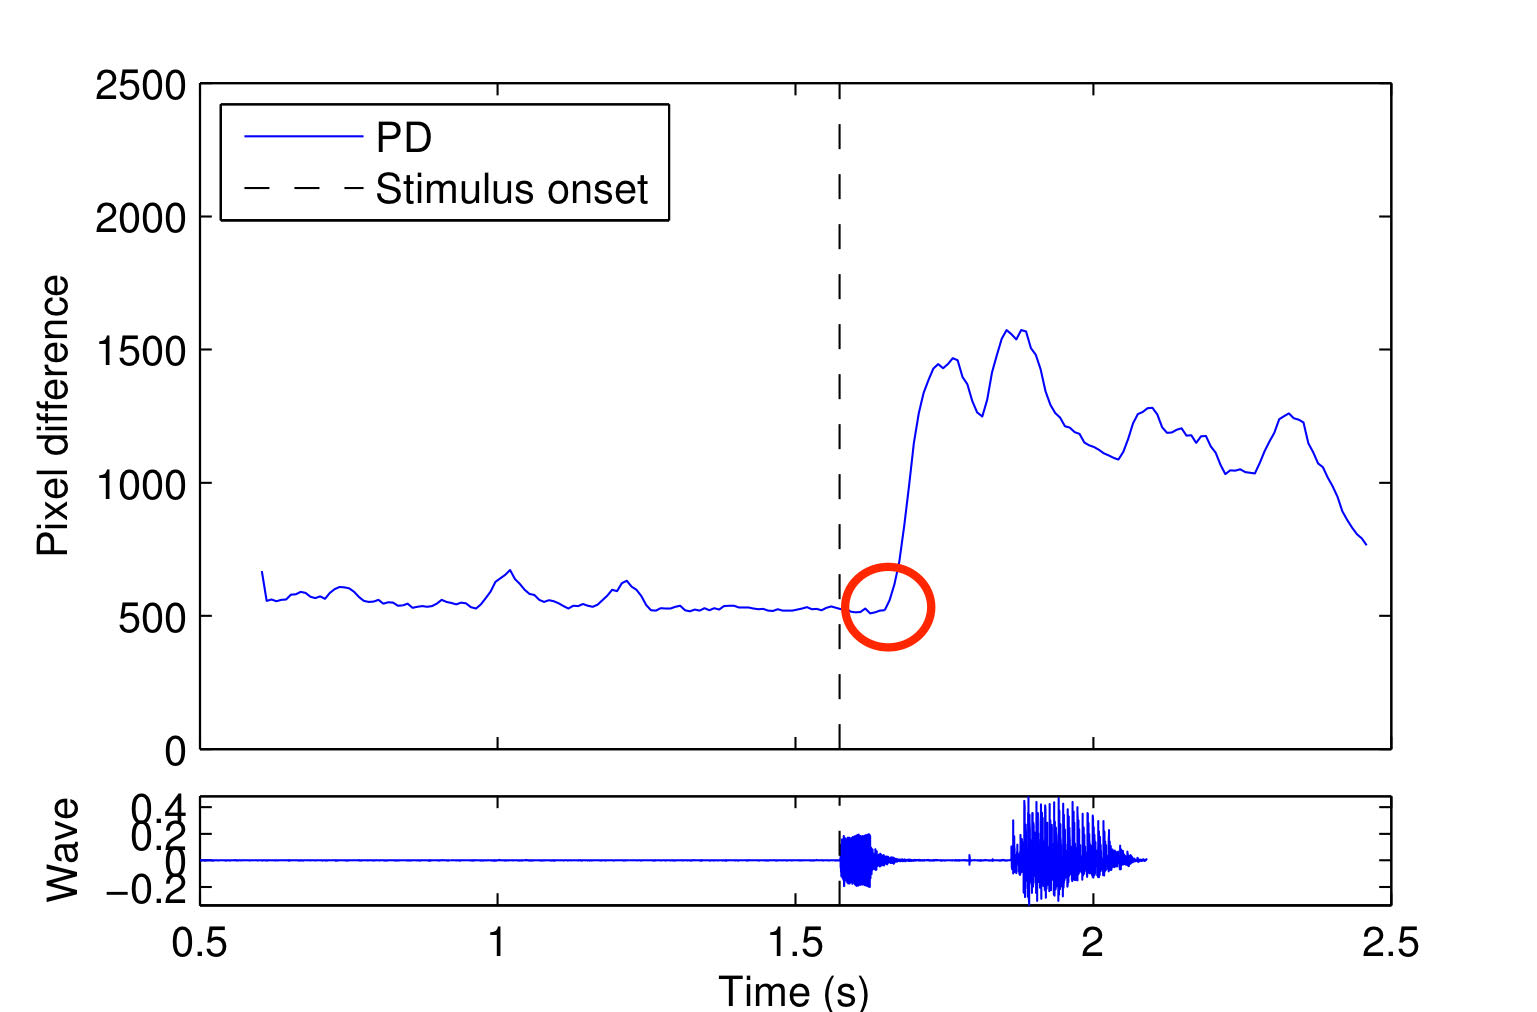
\includegraphics[height=.7\textheight]{figures/pd_caught.jpg}
}

\frame{\frametitle{Pixel Difference (PD): Background}
	\begin{itemize}
		\item The analysis methods presented here are similar to methods
		developed by
		\begin{itemize}
			\item
			 \cite{McMillanCorley-CascadingInfluencesProduction-2010} and
			 \cite{DrakeEtAl-ARTICULATORYEVIDENCEINVOLVEMENT-2013} who used
			 Euclidean distance on ultrasound frames and
			\item \cite{RaeesyEtAl-ParametrisingDegreeArticulator-2011} who
			 used a similar method on MRI data.
		\end{itemize}
		\item The way I have used it, it is actually just the Pythagorean
			theorem applied in a space with a lot more dimensions than~2.
		\end{itemize}
}

\frame{\frametitle{Pixel Difference (PD): Pythagoras (wasn't first)}
	
\begin{columns}
  \begin{column}{5cm}
    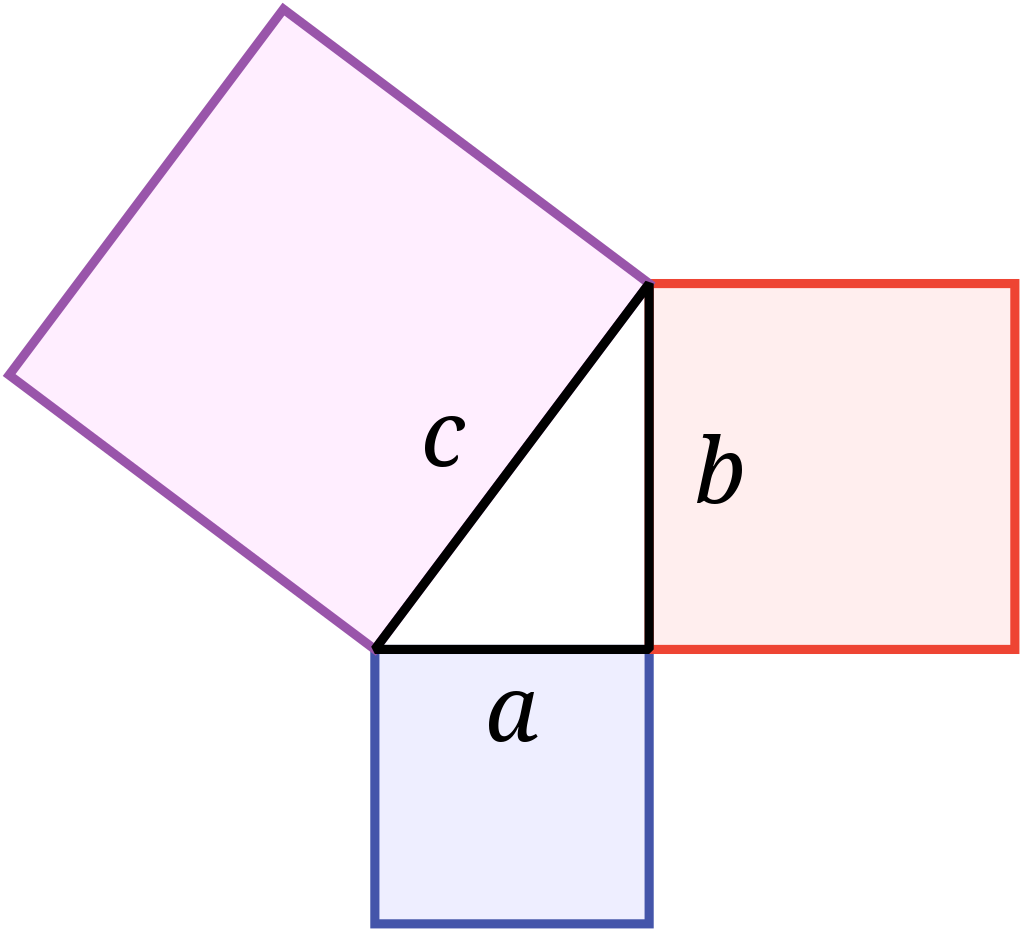
\includegraphics[width=\columnwidth]{figures/1024px-Pythagorean.svg.png}
  \end{column}
  \begin{column}{5cm}
    \centering
    Pythagorean Theorem:
    \begin{equation*}
      a^2 + b^2 = c^2
    \end{equation*}
    \citep{Euclid-ElementsBooksIXIII-2006}
  \end{column}
\end{columns}
\vfill
  {\scriptsize
    By en:User:Wapcaplet - Transwikied from en:. Originally created by
    en:User:Michael Hardy, then scaled, with colour and labels being added by
    en:User:Wapcaplet, transformed in svg format by fr:Utilisateur:Steff, changed
    colors and font by de:Leo2004, CC BY-SA 3.0,
    \url{https://commons.wikimedia.org/w/index.php?curid=640875} 
  }
}

\frame{\frametitle{Pixel Difference (PD): The maths}
	\begin{equation*}
	l2(t+0.5) = \sqrt{\sum_{i, j} (x(i,j,t+1) - x(i,j,t))^2}
	\end{equation*}

	\begin{itemize}
		\item $i$ and $j$ are indices that span the width and height of the
		image, $t$ is the time index.
		\item Like said, this is actually just the Pythagorean theorem applied
		in a space with a lot more dimensions than 2.
	\end{itemize}

	}

\frame{\frametitle{Pixel Difference (PD): The maths visually}
	\centering
	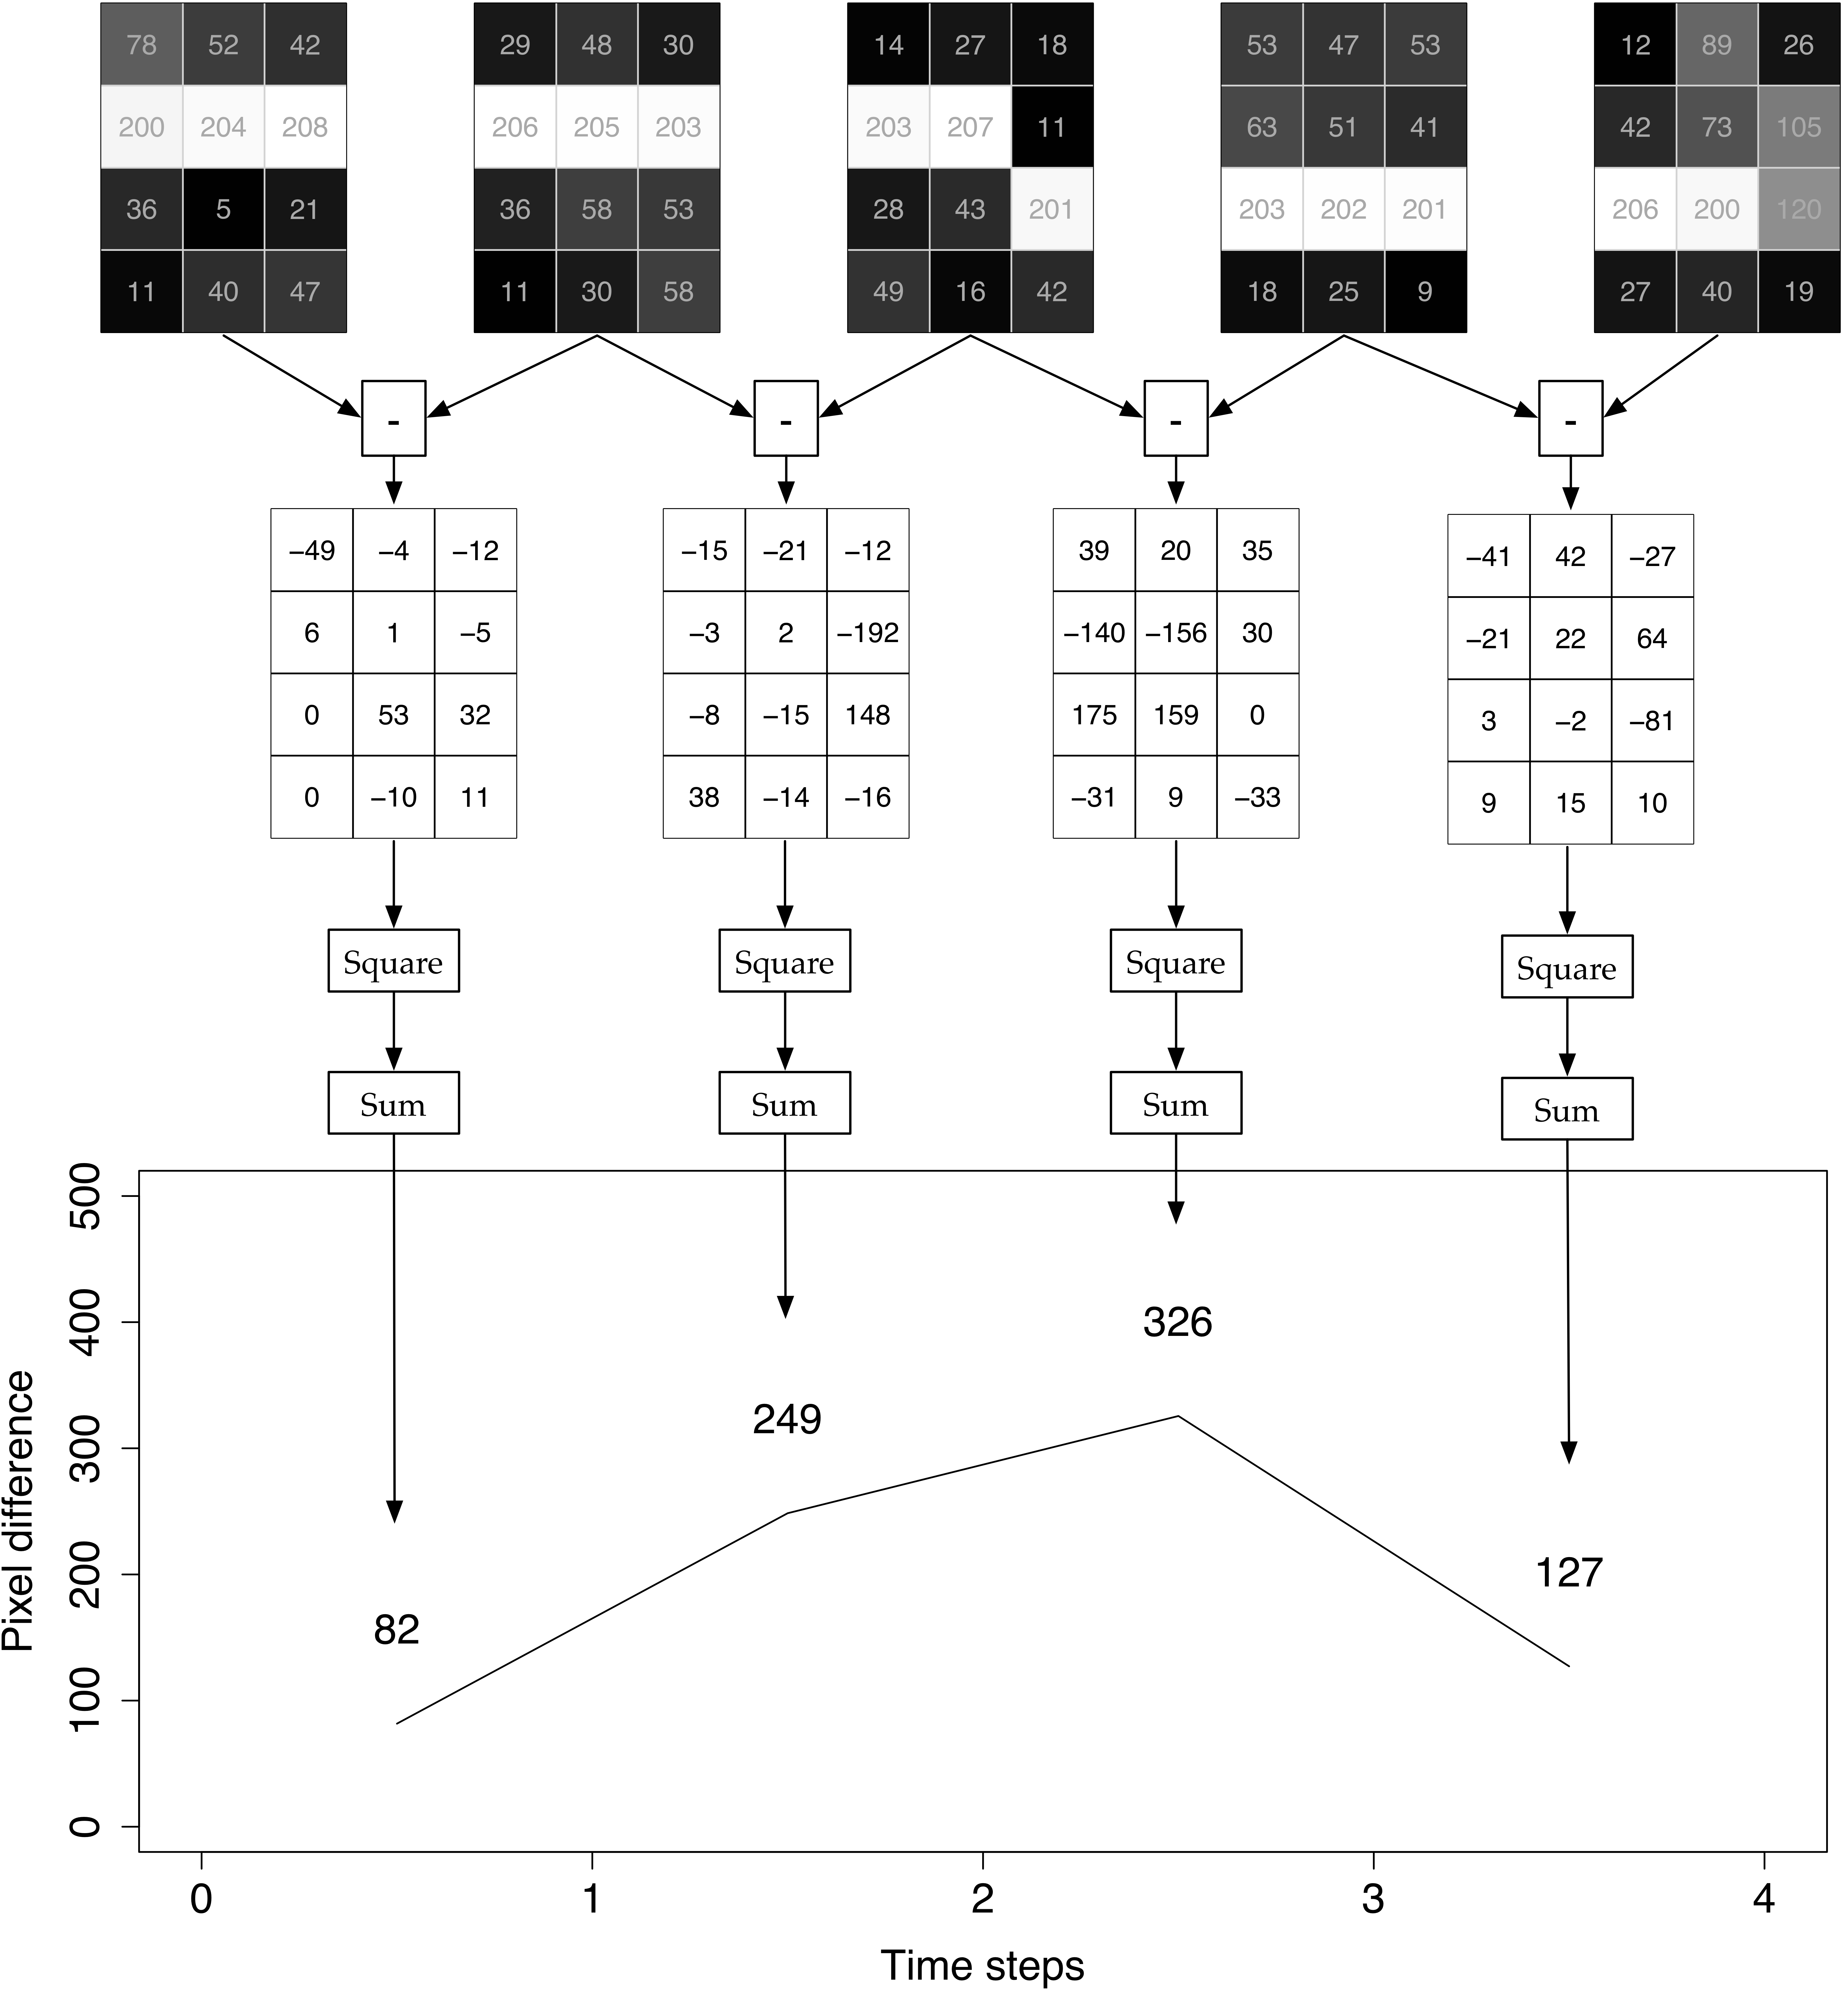
\includegraphics[height=.8\textheight]{figures/pixel_difference_demo_noise_square_sum_tall.png}
}

\frame{
  \centering
  {
    \bf \Large 
    \usebeamercolor[fg]{title}
    \vfill
    Some quick results
    \vfill
%    \includegraphics[height=1.5cm]{figures/aalto_logo} 
  }
}


\frame{\frametitle{Delayed naming results: Articulatory to Acoustic Interval}
	\begin{center}
		\vspace*{-.5cm}
		\hspace*{-1cm}
		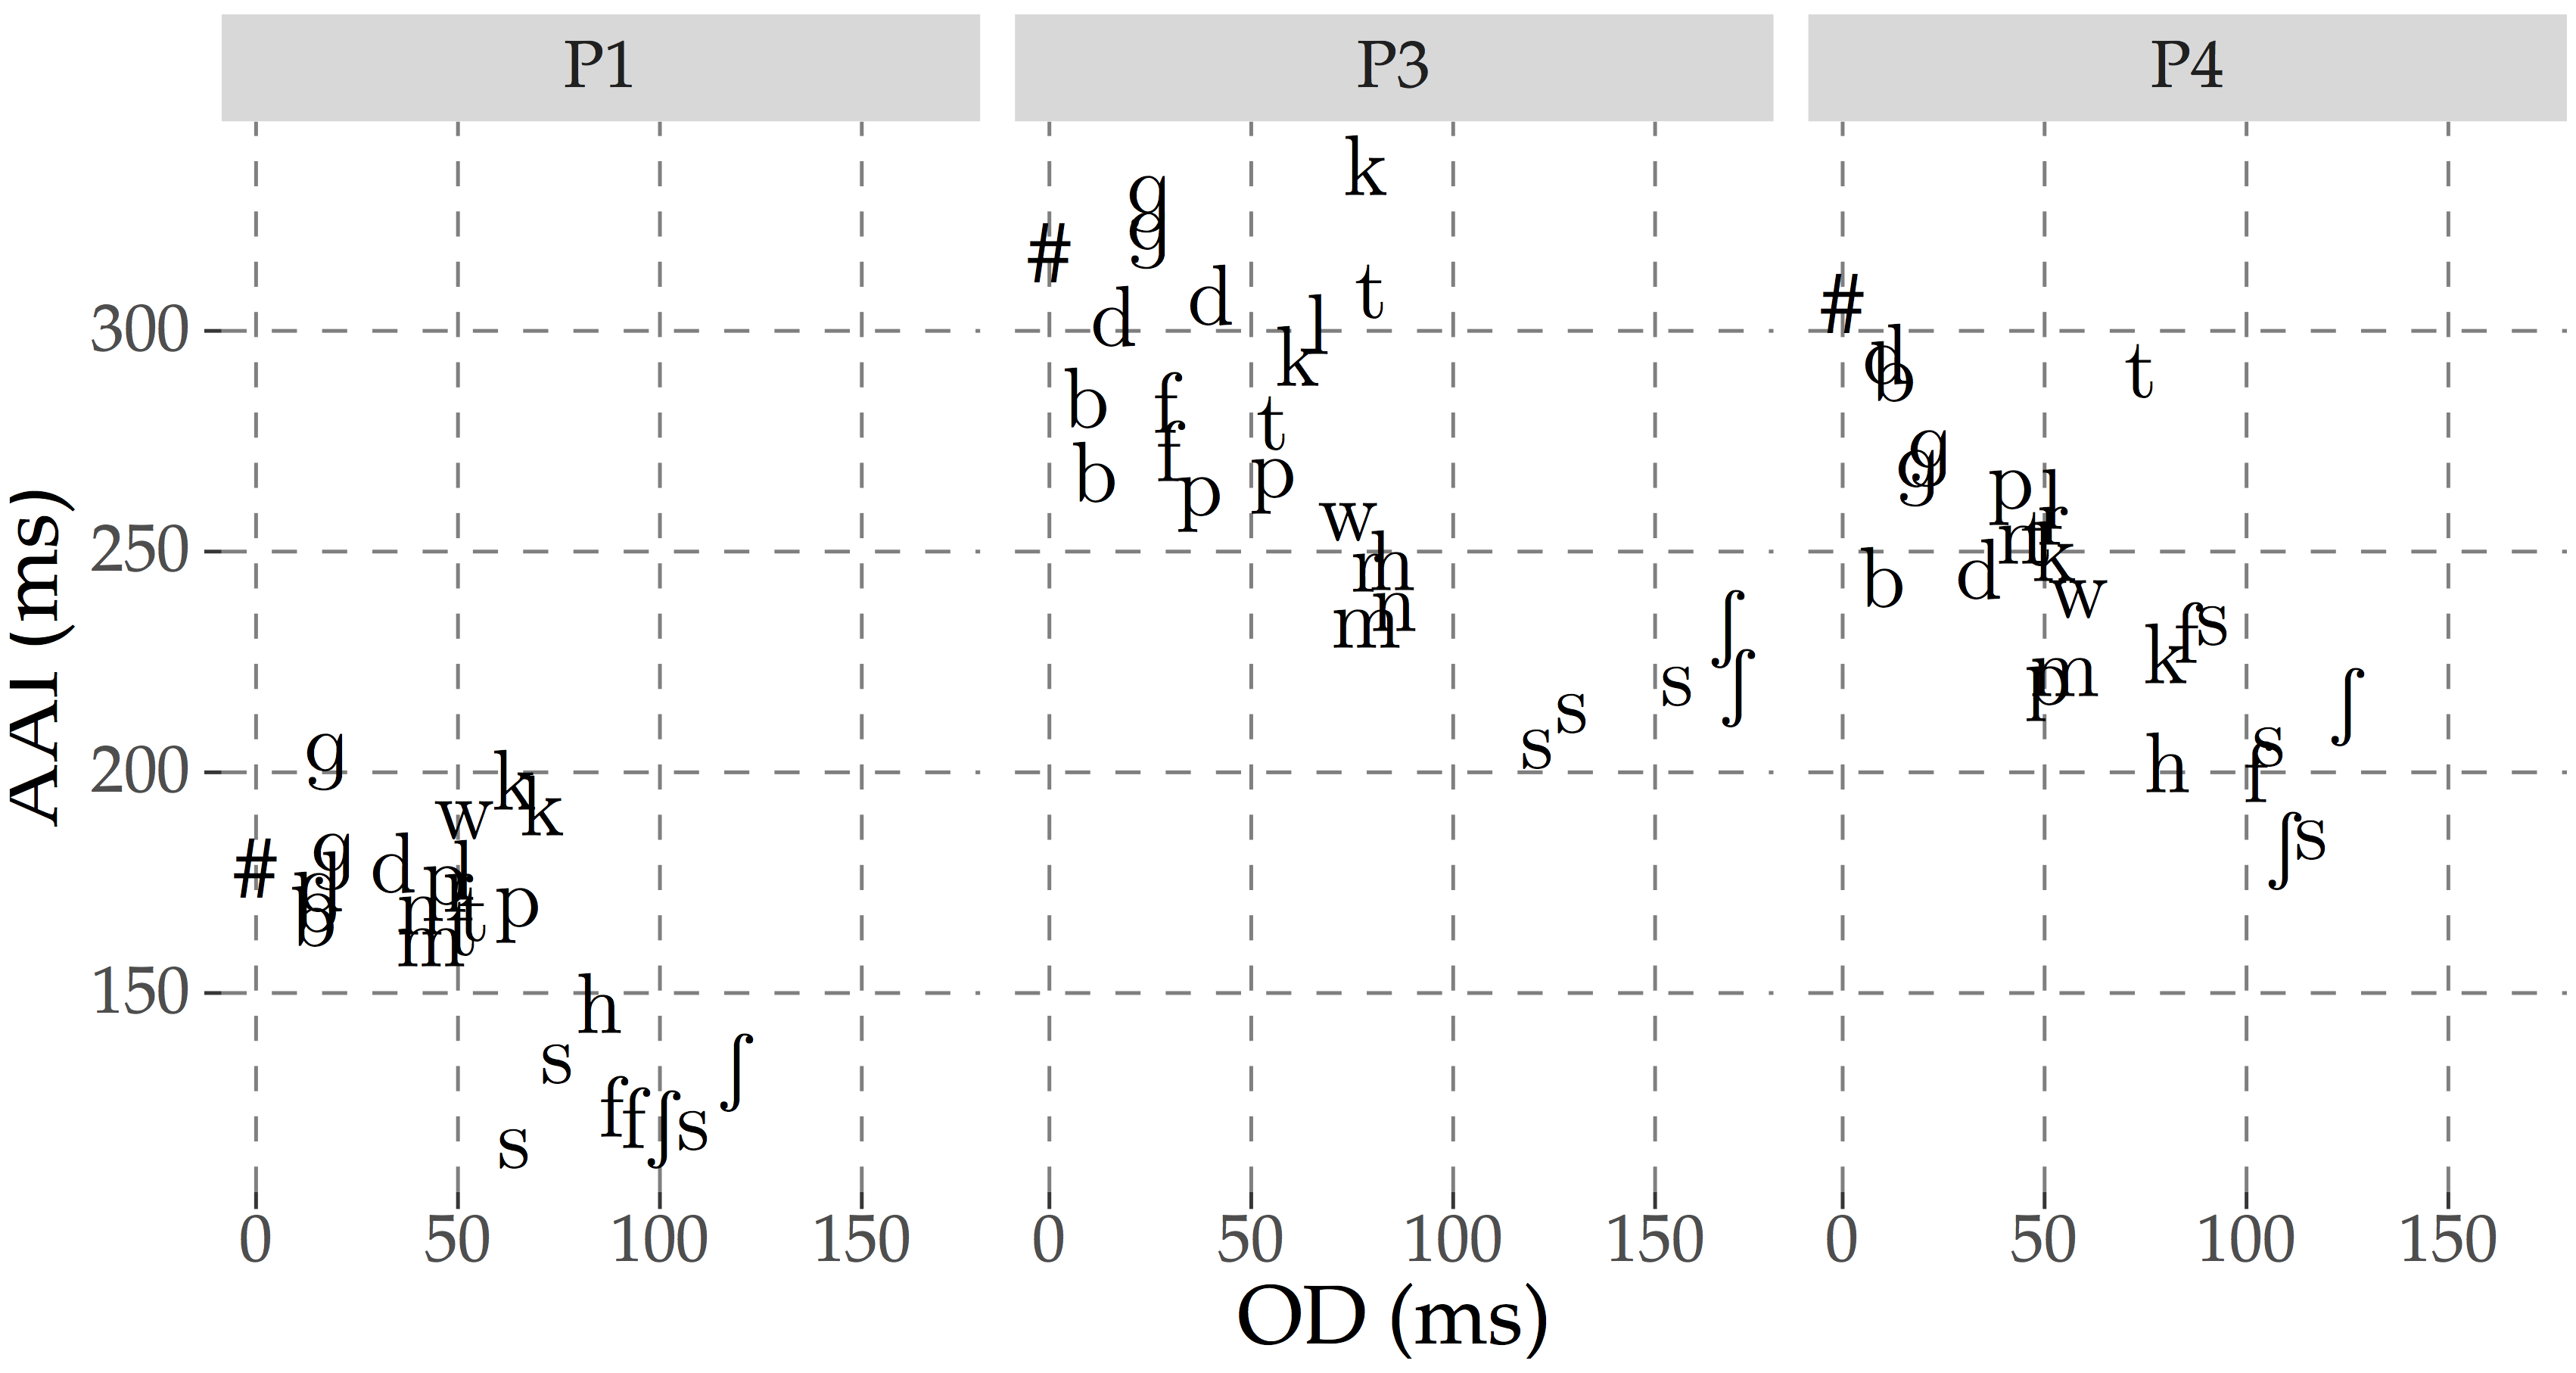
\includegraphics[width=\textwidth]{figures/OD_vs_AAI.jpg}
	\end{center}
	Medianised within participant, over several repetitions and over
	the vowels \textipa{/a,i,O/}. Over all analysable n = 1386: 439 from P1, 672 from P3,
	and 275 from P4.
}

\frame{\frametitle{Theory: Effect of OD on AAI}
	% \begin{itemize}
	% 	\item As the Onset Duration (OD) gets longer, Articulatory to Acoustic
	% 	Interval (AAI) shortens.
	% 	% \item First three lines represent individual utterances, final line is
	% 	% a conceptual model of the effect of continuously lengthening OD.
	% \end{itemize}
	\begin{center}
		\hspace*{-.5cm}
		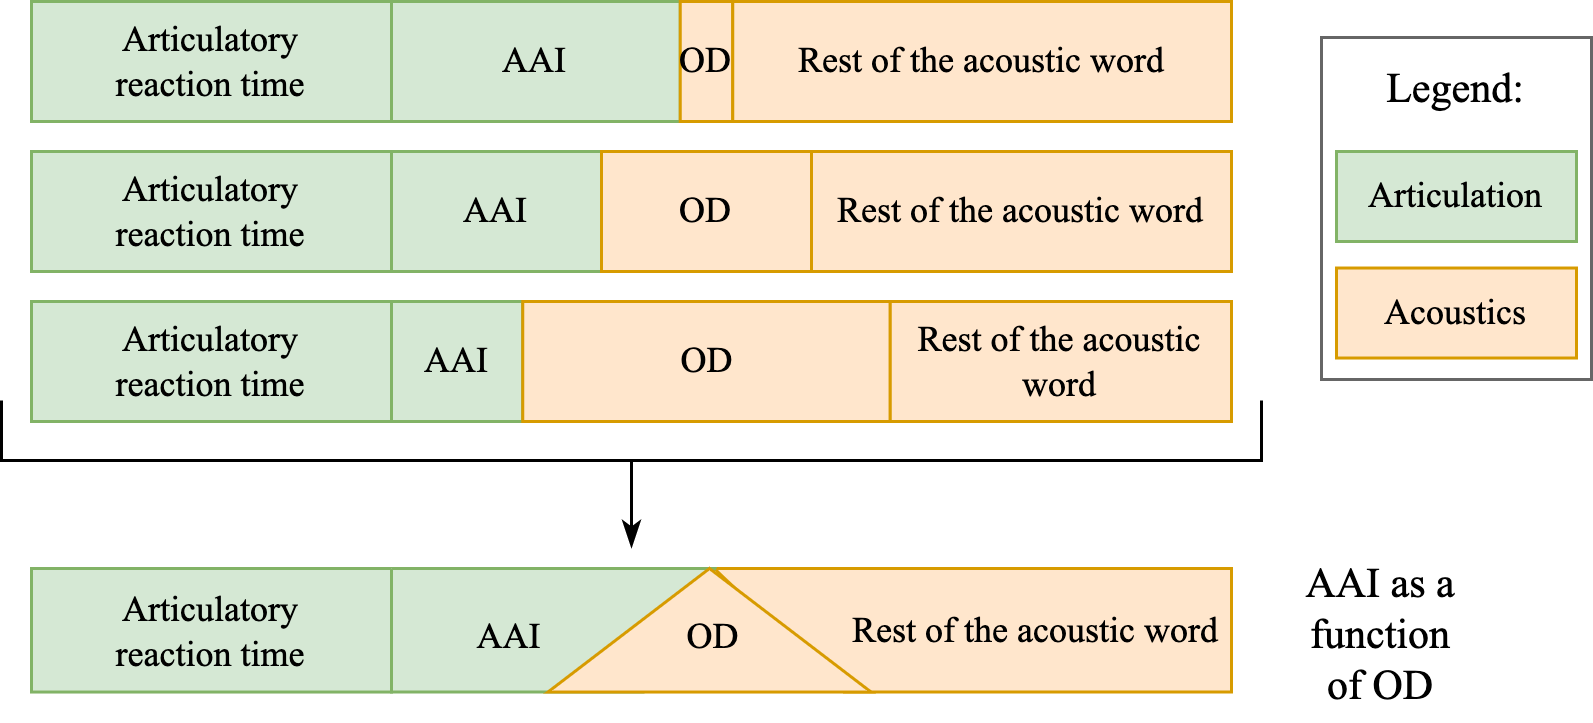
\includegraphics[width=1.1\textwidth]{effect_of_OD.drawio.png}
	\end{center}
}

\frame{\frametitle{Theory: Effect of articulatory rate on AAI}
	% \begin{itemize}
	% 	\item If we keep the utterance content constant but vary articulation
	% 	rate, all parts (AAI, OD, and acoustic word) get longer as articulation
	% 	rate goes down.
	% \end{itemize}
	\begin{center}
		\hspace*{-.5cm}
		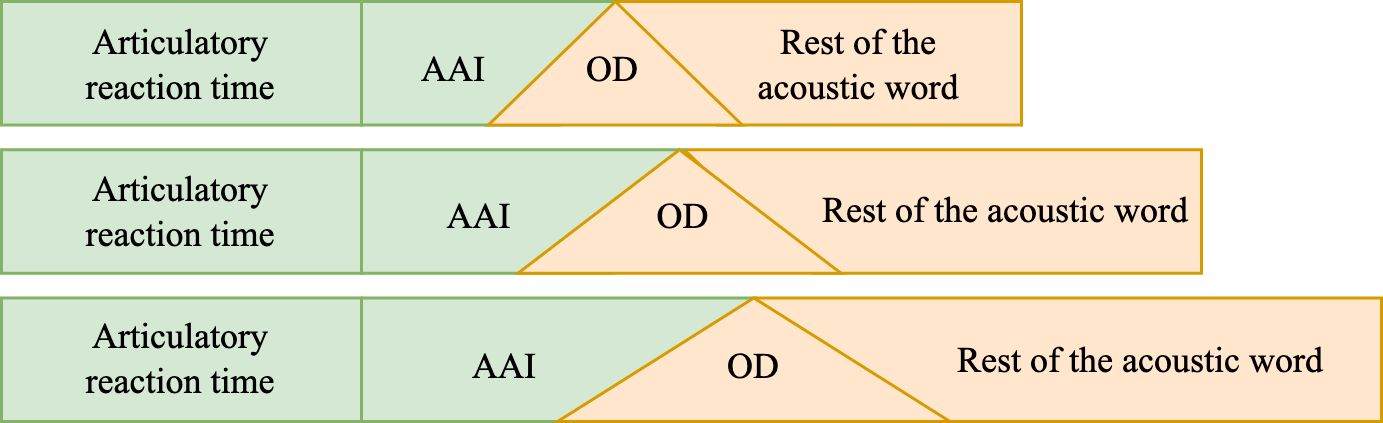
\includegraphics[width=\textwidth]{effect_of_RhymeDur.drawio.png}
	\end{center}
}

\frame{\frametitle{Starting position}
	\begin{itemize}
		\item 'Remain at rest' does not define what 'rest' means.
	\end{itemize}
	\centering
	\hspace*{-.9cm}
	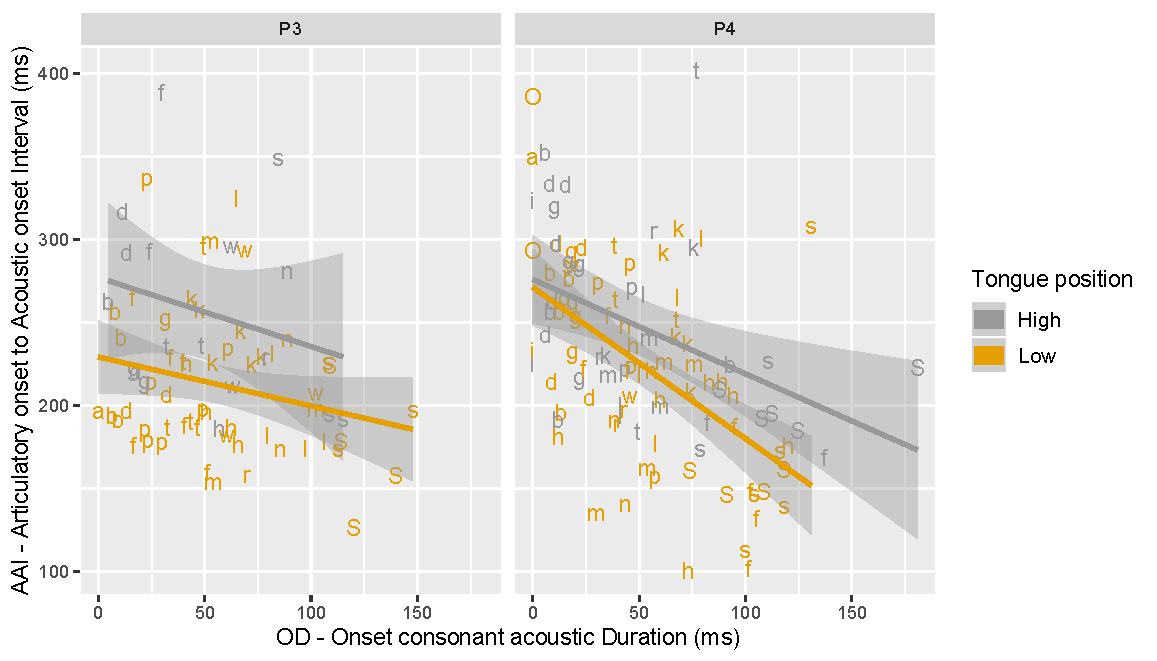
\includegraphics[width=1.17\linewidth]{figures/OD_vs_AAI_smoothsP3P4.pdf}
	% \includegraphics[width=.8\linewidth]{figures/raw_interpolated_2D_step5}
	
}

\frame{
  \centering
  {
    \bf \Large 
    \usebeamercolor[fg]{title}
    \vfill
    Conclusions
    \vfill
%    \includegraphics[height=1.5cm]{figures/aalto_logo} 
  }
}

\frame{\frametitle{Conclusions}
Speech initiation:
\begin{itemize}
  \item It's a lot more complex than I would have thought almost 12 years ago.
  \item The results in this talk rest on samples that aren't terribly big and
  don't span too many languages (but aren't based in just English).
\end{itemize}
\vfill
Methods:
  \begin{itemize}
		\item We don't always need to look to super complicated tools to actually
		make a drastic improvement in a workflow.
    \item We should always spare at least a short moment to think about methods
    -- arguably even when doing a 1:1 replication of a previous study.
    \item We should try to find a balance between doubting our methods and just
    getting on with the work.
	\end{itemize}

	}

\frame{\frametitle{Pixel Difference (PD): The maths visually}
	\centering
	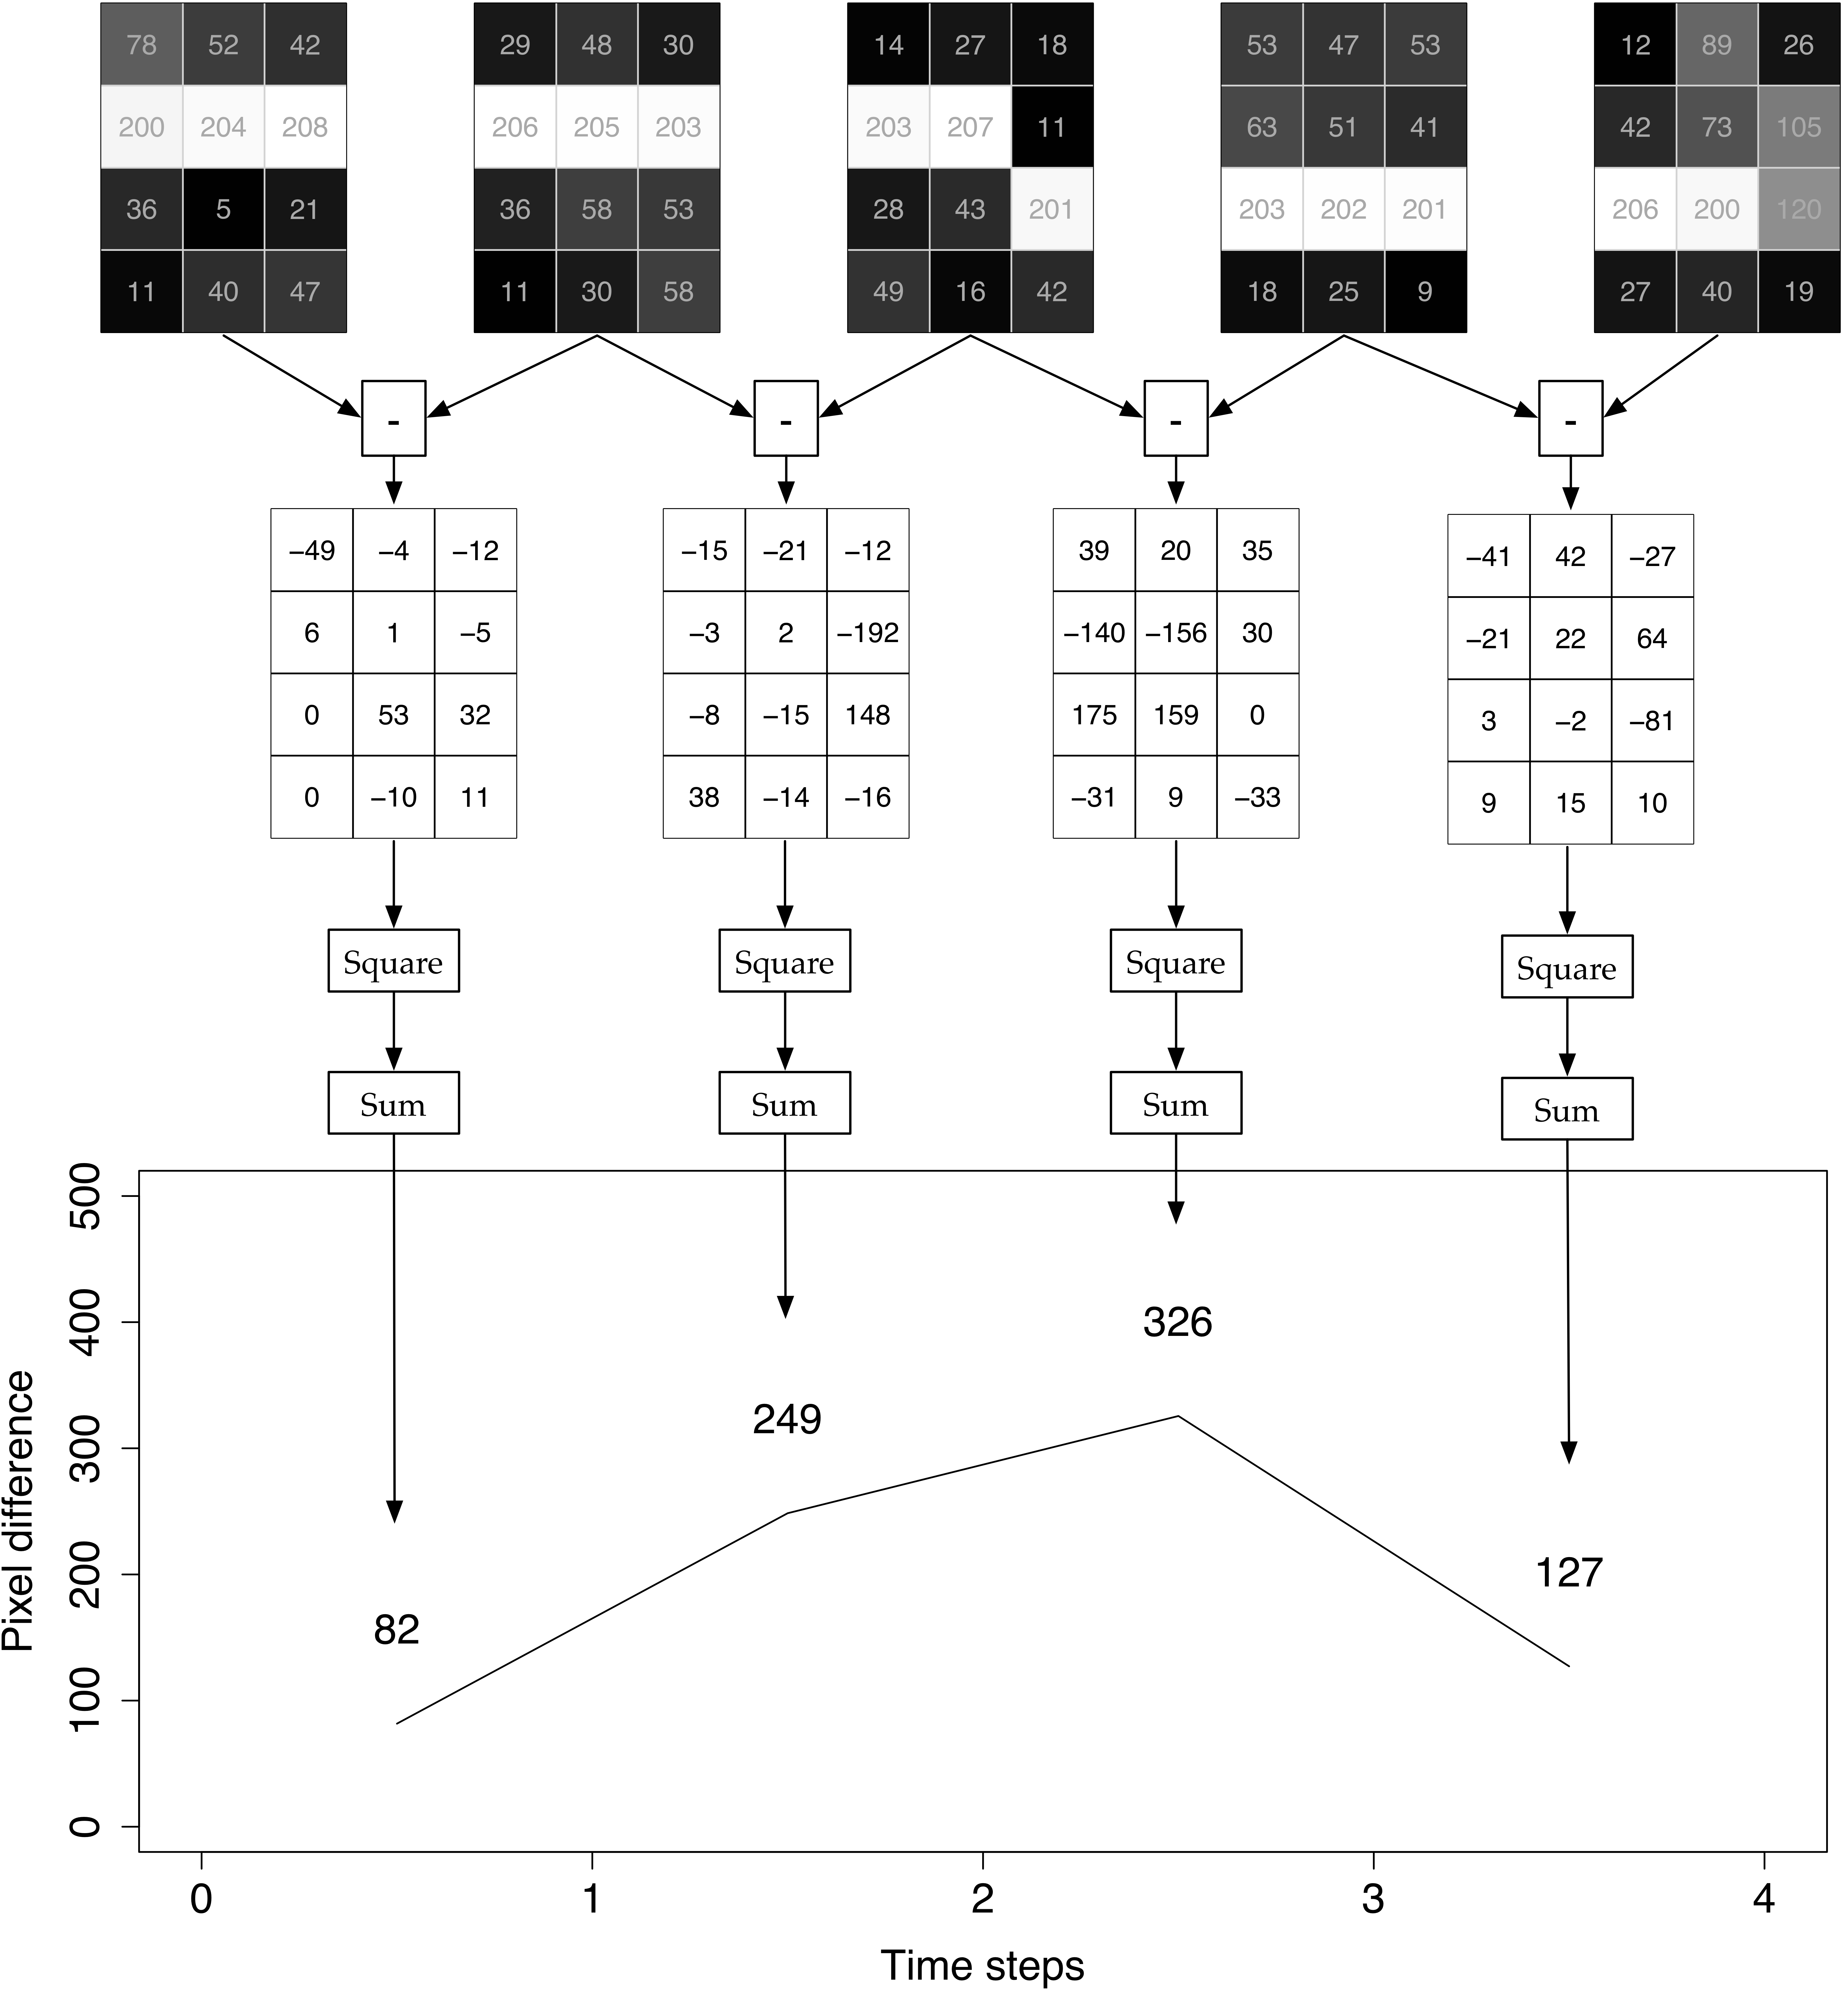
\includegraphics[height=.8\textheight]{figures/pixel_difference_demo_noise_square_sum_tall.png}
}

\frame{
  \centering
  {
    \bf \Large 
    \usebeamercolor[fg]{title}
    Thank you! Questions?
    
    \vfill
%    \includegraphics[height=1.5cm]{figures/aalto_logo} 
  }
}

\frame{\frametitle{References}
  \tiny
  \bibliographystyle{apalike}
  \bibliography{main}
}


\end{document}

